%% bare_conf.tex
%% V1.4a
%% 2014/09/17
%% by Michael Shell
%% See:
%% http://www.michaelshell.org/
%% for current contact information.
%%
%% This is a skeleton file demonstrating the use of IEEEtran.cls
%% (requires IEEEtran.cls version 1.8a or later) with an IEEE
%% conference paper.
%%
%% Support sites:
%% http://www.michaelshell.org/tex/ieeetran/
%% http://www.ctan.org/tex-archive/macros/latex/contrib/IEEEtran/
%% and
%% http://www.ieee.org/

%%*************************************************************************
%% Legal Notice:
%% This code is offered as-is without any warranty either expressed or
%% implied; without even the implied warranty of MERCHANTABILITY or
%% FITNESS FOR A PARTICULAR PURPOSE!
%% User assumes all risk.
%% In no event shall IEEE or any contributor to this code be liable for
%% any damages or losses, including, but not limited to, incidental,
%% consequential, or any other damages, resulting from the use or misuse
%% of any information contained here.
%%
%% All comments are the opinions of their respective authors and are not
%% necessarily endorsed by the IEEE.
%%
%% This work is distributed under the LaTeX Project Public License (LPPL)
%% ( http://www.latex-project.org/ ) version 1.3, and may be freely used,
%% distributed and modified. A copy of the LPPL, version 1.3, is included
%% in the base LaTeX documentation of all distributions of LaTeX released
%% 2003/12/01 or later.
%% Retain all contribution notices and credits.
%% ** Modified files should be clearly indicated as such, including  **
%% ** renaming them and changing author support contact information. **
%%
%% File list of work: IEEEtran.cls, IEEEtran_HOWTO.pdf, bare_adv.tex,
%%                    bare_conf.tex, bare_jrnl.tex, bare_conf_compsoc.tex,
%%                    bare_jrnl_compsoc.tex, bare_jrnl_transmag.tex
%%*************************************************************************


% *** Authors should verify (and, if needed, correct) their LaTeX system  ***
% *** with the testflow diagnostic prior to trusting their LaTeX platform ***
% *** with production work. IEEE's font choices and paper sizes can       ***
% *** trigger bugs that do not appear when using other class files.       ***                          ***
% The testflow support page is at:
% http://www.michaelshell.org/tex/testflow/



\documentclass[conference]{IEEEtran}
% Some Computer Society conferences also require the compsoc mode option,
% but others use the standard conference format.
%
% If IEEEtran.cls has not been installed into the LaTeX system files,
% manually specify the path to it like:
% \documentclass[conference]{../sty/IEEEtran}





% Some very useful LaTeX packages include:
% (uncomment the ones you want to load)


% *** MISC UTILITY PACKAGES ***
%
%\usepackage{ifpdf}
% Heiko Oberdiek's ifpdf.sty is very useful if you need conditional
% compilation based on whether the output is pdf or dvi.
% usage:
% \ifpdf
%   % pdf code
% \else
%   % dvi code
% \fi
% The latest version of ifpdf.sty can be obtained from:
% http://www.ctan.org/tex-archive/macros/latex/contrib/oberdiek/
% Also, note that IEEEtran.cls V1.7 and later provides a builtin
% \ifCLASSINFOpdf conditional that works the same way.
% When switching from latex to pdflatex and vice-versa, the compiler may
% have to be run twice to clear warning/error messages.






% *** CITATION PACKAGES ***
%
%\usepackage{cite}
% cite.sty was written by Donald Arseneau
% V1.6 and later of IEEEtran pre-defines the format of the cite.sty package
% \cite{} output to follow that of IEEE. Loading the cite package will
% result in citation numbers being automatically sorted and properly
% "compressed/ranged". e.g., [1], [9], [2], [7], [5], [6] without using
% cite.sty will become [1], [2], [5]--[7], [9] using cite.sty. cite.sty's
% \cite will automatically add leading space, if needed. Use cite.sty's
% noadjust option (cite.sty V3.8 and later) if you want to turn this off
% such as if a citation ever needs to be enclosed in parenthesis.
% cite.sty is already installed on most LaTeX systems. Be sure and use
% version 5.0 (2009-03-20) and later if using hyperref.sty.
% The latest version can be obtained at:
% http://www.ctan.org/tex-archive/macros/latex/contrib/cite/
% The documentation is contained in the cite.sty file itself.






% *** GRAPHICS RELATED PACKAGES ***
%
\ifCLASSINFOpdf
  \usepackage[pdftex]{graphicx}
  %declare the path(s) where your graphic files are
  \graphicspath{{./}}
  %and their extensions so you won't have to specify these with
  %every instance of \includegraphics
  \DeclareGraphicsExtensions{.pdf,.jpeg,.png}
\else
  % or other class option (dvipsone, dvipdf, if not using dvips). graphicx
  % will default to the driver specified in the system graphics.cfg if no
  % driver is specified.
  % \usepackage[dvips]{graphicx}
  % declare the path(s) where your graphic files are
  % \graphicspath{{../eps/}}
  % and their extensions so you won't have to specify these with
  % every instance of \includegraphics
  % \DeclareGraphicsExtensions{.eps}
\fi
% graphicx was written by David Carlisle and Sebastian Rahtz. It is
% required if you want graphics, photos, etc. graphicx.sty is already
% installed on most LaTeX systems. The latest version and documentation
% can be obtained at:
% http://www.ctan.org/tex-archive/macros/latex/required/graphics/
% Another good source of documentation is "Using Imported Graphics in
% LaTeX2e" by Keith Reckdahl which can be found at:
% http://www.ctan.org/tex-archive/info/epslatex/
%
% latex, and pdflatex in dvi mode, support graphics in encapsulated
% postscript (.eps) format. pdflatex in pdf mode supports graphics
% in .pdf, .jpeg, .png and .mps (metapost) formats. Users should ensure
% that all non-photo figures use a vector format (.eps, .pdf, .mps) and
% not a bitmapped formats (.jpeg, .png). IEEE frowns on bitmapped formats
% which can result in "jaggedy"/blurry rendering of lines and letters as
% well as large increases in file sizes.
%
% You can find documentation about the pdfTeX application at:
% http://www.tug.org/applications/pdftex





% *** MATH PACKAGES ***
%
%\usepackage[cmex10]{amsmath}
\usepackage{amssymb}
% A popular package from the American Mathematical Society that provides
% many useful and powerful commands for dealing with mathematics. If using
% it, be sure to load this package with the cmex10 option to ensure that
% only type 1 fonts will utilized at all point sizes. Without this option,
% it is possible that some math symbols, particularly those within
% footnotes, will be rendered in bitmap form which will result in a
% document that can not be IEEE Xplore compliant!
%
% Also, note that the amsmath package sets \interdisplaylinepenalty to 10000
% thus preventing page breaks from occurring within multiline equations. Use:
%\interdisplaylinepenalty=2500
% after loading amsmath to restore such page breaks as IEEEtran.cls normally
% does. amsmath.sty is already installed on most LaTeX systems. The latest
% version and documentation can be obtained at:
% http://www.ctan.org/tex-archive/macros/latex/required/amslatex/math/





% *** SPECIALIZED LIST PACKAGES ***
%
%\usepackage{algorithmic}
% algorithmic.sty was written by Peter Williams and Rogerio Brito.
% This package provides an algorithmic environment fo describing algorithms.
% You can use the algorithmic environment in-text or within a figure
% environment to provide for a floating algorithm. Do NOT use the algorithm
% floating environment provided by algorithm.sty (by the same authors) or
% algorithm2e.sty (by Christophe Fiorio) as IEEE does not use dedicated
% algorithm float types and packages that provide these will not provide
% correct IEEE style captions. The latest version and documentation of
% algorithmic.sty can be obtained at:
% http://www.ctan.org/tex-archive/macros/latex/contrib/algorithms/
% There is also a support site at:
% http://algorithms.berlios.de/index.html
% Also of interest may be the (relatively newer and more customizable)
% algorithmicx.sty package by Szasz Janos:
% http://www.ctan.org/tex-archive/macros/latex/contrib/algorithmicx/




% *** ALIGNMENT PACKAGES ***
%
%\usepackage{array}
% Frank Mittelbach's and David Carlisle's array.sty patches and improves
% the standard LaTeX2e array and tabular environments to provide better
% appearance and additional user controls. As the default LaTeX2e table
% generation code is lacking to the point of almost being broken with
% respect to the quality of the end results, all users are strongly
% advised to use an enhanced (at the very least that provided by array.sty)
% set of table tools. array.sty is already installed on most systems. The
% latest version and documentation can be obtained at:
% http://www.ctan.org/tex-archive/macros/latex/required/tools/


% IEEEtran contains the IEEEeqnarray family of commands that can be used to
% generate multiline equations as well as matrices, tables, etc., of high
% quality.




% *** SUBFIGURE PACKAGES ***
%\ifCLASSOPTIONcompsoc
%  \usepackage[caption=false,font=normalsize,labelfont=sf,textfont=sf]{subfig}
%\else
%  \usepackage[caption=false,font=footnotesize]{subfig}
%\fi
% subfig.sty, written by Steven Douglas Cochran, is the modern replacement
% for subfigure.sty, the latter of which is no longer maintained and is
% incompatible with some LaTeX packages including fixltx2e. However,
% subfig.sty requires and automatically loads Axel Sommerfeldt's caption.sty
% which will override IEEEtran.cls' handling of captions and this will result
% in non-IEEE style figure/table captions. To prevent this problem, be sure
% and invoke subfig.sty's "caption=false" package option (available since
% subfig.sty version 1.3, 2005/06/28) as this is will preserve IEEEtran.cls
% handling of captions.
% Note that the Computer Society format requires a larger sans serif font
% than the serif footnote size font used in traditional IEEE formatting
% and thus the need to invoke different subfig.sty package options depending
% on whether compsoc mode has been enabled.
%
% The latest version and documentation of subfig.sty can be obtained at:
% http://www.ctan.org/tex-archive/macros/latex/contrib/subfig/




% *** FLOAT PACKAGES ***
%
%\usepackage{fixltx2e}
% fixltx2e, the successor to the earlier fix2col.sty, was written by
% Frank Mittelbach and David Carlisle. This package corrects a few problems
% in the LaTeX2e kernel, the most notable of which is that in current
% LaTeX2e releases, the ordering of single and double column floats is not
% guaranteed to be preserved. Thus, an unpatched LaTeX2e can allow a
% single column figure to be placed prior to an earlier double column
% figure. The latest version and documentation can be found at:
% http://www.ctan.org/tex-archive/macros/latex/base/


%\usepackage{stfloats}
% stfloats.sty was written by Sigitas Tolusis. This package gives LaTeX2e
% the ability to do double column floats at the bottom of the page as well
% as the top. (e.g., "\begin{figure*}[!b]" is not normally possible in
% LaTeX2e). It also provides a command:
%\fnbelowfloat
% to enable the placement of footnotes below bottom floats (the standard
% LaTeX2e kernel puts them above bottom floats). This is an invasive package
% which rewrites many portions of the LaTeX2e float routines. It may not work
% with other packages that modify the LaTeX2e float routines. The latest
% version and documentation can be obtained at:
% http://www.ctan.org/tex-archive/macros/latex/contrib/sttools/
% Do not use the stfloats baselinefloat ability as IEEE does not allow
% \baselineskip to stretch. Authors submitting work to the IEEE should note
% that IEEE rarely uses double column equations and that authors should try
% to avoid such use. Do not be tempted to use the cuted.sty or midfloat.sty
% packages (also by Sigitas Tolusis) as IEEE does not format its papers in
% such ways.
% Do not attempt to use stfloats with fixltx2e as they are incompatible.
% Instead, use Morten Hogholm'a dblfloatfix which combines the features
% of both fixltx2e and stfloats:
%
% \usepackage{dblfloatfix}
% The latest version can be found at:
% http://www.ctan.org/tex-archive/macros/latex/contrib/dblfloatfix/




% *** PDF, URL AND HYPERLINK PACKAGES ***
%
%\usepackage{url}
% url.sty was written by Donald Arseneau. It provides better support for
% handling and breaking URLs. url.sty is already installed on most LaTeX
% systems. The latest version and documentation can be obtained at:
% http://www.ctan.org/tex-archive/macros/latex/contrib/url/
% Basically, \url{my_url_here}.




% *** Do not adjust lengths that control margins, column widths, etc. ***
% *** Do not use packages that alter fonts (such as pslatex).         ***
% There should be no need to do such things with IEEEtran.cls V1.6 and later.
% (Unless specifically asked to do so by the journal or conference you plan
% to submit to, of course. )


% correct bad hyphenation here
\hyphenation{op-tical net-works semi-conduc-tor}


\begin{document}
%
% paper title
% Titles are generally capitalized except for words such as a, an, and, as,
% at, but, by, for, in, nor, of, on, or, the, to and up, which are usually
% not capitalized unless they are the first or last word of the title.
% Linebreaks \\ can be used within to get better formatting as desired.
% Do not put math or special symbols in the title.
\title{Literature Review \\
Efficient KNN Join Algorithms}


% author names and affiliations
% use a multiple column layout for up to three different
% affiliations
\author{\IEEEauthorblockN{Ramanathan Sivagurunathan}
\IEEEauthorblockA{Sydney University\\
Sydney\\
Email: rsiv5112@syd.uni.edu}}

% conference papers do not typically use \thanks and this command
% is locked out in conference mode. If really needed, such as for
% the acknowledgment of grants, issue a \IEEEoverridecommandlockouts
% after \documentclass

% for over three affiliations, or if they all won't fit within the width
% of the page, use this alternative format:
%
%\author{\IEEEauthorblockN{Michael Shell\IEEEauthorrefmark{1},
%Homer Simpson\IEEEauthorrefmark{2},
%James Kirk\IEEEauthorrefmark{3},
%Montgomery Scott\IEEEauthorrefmark{3} and
%Eldon Tyrell\IEEEauthorrefmark{4}}
%\IEEEauthorblockA{\IEEEauthorrefmark{1}School of Electrical and Computer Engineering\\
%Georgia Institute of Technology,
%Atlanta, Georgia 30332--0250\\ Email: see http://www.michaelshell.org/contact.html}
%\IEEEauthorblockA{\IEEEauthorrefmark{2}Twentieth Century Fox, Springfield, USA\\
%Email: homer@thesimpsons.com}
%\IEEEauthorblockA{\IEEEauthorrefmark{3}Starfleet Academy, San Francisco, California 96678-2391\\
%Telephone: (800) 555--1212, Fax: (888) 555--1212}
%\IEEEauthorblockA{\IEEEauthorrefmark{4}Tyrell Inc., 123 Replicant Street, Los Angeles, California 90210--4321}}




% use for special paper notices
%\IEEEspecialpapernotice{(Invited Paper)}




% make the title area
\maketitle

% As a general rule, do not put math, special symbols or citations
% in the abstract
\begin{abstract}
Review of all available works in KNN Join and their current relevance
in the age of big data and distributed computing
\end{abstract}

% no keywords




% For peer review papers, you can put extra information on the cover
% page as needed:
% \ifCLASSOPTIONpeerreview
% \begin{center} \bfseries EDICS Category: 3-BBND \end{center}
% \fi
%
% For peerreview papers, this IEEEtran command inserts a page break and
% creates the second title. It will be ignored for other modes.
\IEEEpeerreviewmaketitle



\section{Introduction}
% no \IEEEPARstart

KNN (K Nearest Neighbour) is one of the simplest and elegant
classification or regression algorithm which works remarkably well in
practice. It is a non parametric lazy learning algorithm. It is
classified as one of the top 10 machine learning algorithm. KNN Join
has become an important primitive in datamining and
finds its application in multimedia data retrieval, DNA search,
Molecular Biology  and
many other fields. It finds K similar points among the given
dataset. Given all the benefits of KNN there are no efficient
implementation for distributed dataset present in any machine learning
libraries like apache mahout and spark mllib

\section{KNN Join}

\emph{Definition:1} Given two datasets R and S, where $R\ \epsilon\
\mathbb{R}^d\ and\ S\ \epsilon\ \mathbb{R}^d$, KNN Join returns the K
Nearest points in S for every point in R.

\bigskip
     $KNN(R,S) = {(r, KNN(r,S), \forall r\ \epsilon\ \mathbb{R}^d)}$
\bigskip

\emph{Definition:2} Given two datasets R and S where $R\ \epsilon\
\mathbb{R}^d\ and S\ \epsilon\ \mathbb{R}^d$, Approximate KNN Join returns the K
approximate neighbours in S for every point in R.

If $p$ is the exact K\textsuperscript{th} neighbour of r and $p'$ be approximate
K\textsuperscript{th} neighbour of r, then for any $\epsilon$

\bigskip

$d(p,r) <= d(p',r) <= (1+\epsilon) d(p,r)$

\bigskip

The computational complexity of KNN Join is
$O(\|R\| \times \|S\|)$. KNN Join is computationally intensive process, which
is the reason why it is difficult to be used in any application where
the number of elements in set R and S is large. Until late 90s KNN was
never considered a feasible algorithm at all due to its
complexity. There is lot work has been done to reduce the
computational complexity. Pre Big data era, algorithms were focussing
on either Indexing Method or Paritioning Method in a centralized
setup. In this modern day of high velocity and volume of data, only distributed
approach will yield the results in resonable amount of time.

\bigskip

\begin{table}[!t]
%\renewcommand{\arraystretch}{1.3}
\caption{Notations}
\label{notations}
\centering
\begin{tabular}{|c|l|}
\hline
Notation & Meaning \\
\hline
R and S & Dataset\\

k & Number of neighbour points \\

d & Number of dimensions \\

n & Number of elements in Dataset \\

c & some positive constant \\

r,s & points in Dataset \\

d(r,s) & Distance between two points r and s \\

$O_i$ & Pivot points \\

\hline
\end{tabular}
\end{table}

\subsection{Methods}
The various algorithms to solve the computational complexity
falls into one or two of these two methodology.
\begin{enumerate}
\item Index Based
\item Partition Based
\end{enumerate}

In Index based KNN Join, an index is created for both R and S
dataset. Index is used a primary way of reducing complexity in \cite{jagadish_idistance:_2005}
\cite{yu_efficient_2007} \cite{mux}. In distance based index
\cite{jagadish_idistance:_2005} the number of comparison for every
query can be as low as $log(n)$, where n is the number of element is
dataset S.

Using index for reducing distance compuation with every element, works
well for 2D or 3D geospatial data, but the major drawback with the
index based approach is that when the number of dimensions increase
creating an index is much costly and its performance is similar to
sequential scan. This is because at higher dimensions the distance
between closest and farthest neighbors will be nearly same
\cite{beyer_when_1999}. One key problem with this approach is when
data is distributed it is difficult to create an index.

\bigskip

In Partition based KNN Join, the dataset is partitioned into different
partitions and for each partition in R only few partitions in S which are
near to R is considered for presence of Nearest Neighbours. The
partition can be distance based or hashing based. This
method quickly simplifies the number of distance calculations. This method is followed in
\cite{lu_efficient_2012}, \cite{stupar_rankreduceprocessing_2010}. One
of the main challenge is to get all nearby neighbours for a subset
$R_i$ in relatively few subsets of $S_i$.

\bigskip

\subsection{Centralised vs Distributed}

Since most work in KNN Join has been done before the big data era,
the main limitations of most algorithms are that being centralised
\cite{jagadish_idistance:_2005}.
Several recent studies \cite{stupar_rankreduceprocessing_2010},
\cite{lu_efficient_2012} have focused on distributed
processing, which enables those algorithms to be used in bigger
dataset which is not possible otherwise.

Hadoop Mapreduce was dominant framework for past 10 years. But as the
systems evolve, mapreduce framework is on the way out
too. Now spark is quickly becoming the defacto framework for
distributed computing. There is significant increase in number users
in spark and it has proved its exceptional performance over
hadoop. But there are no work that has been done to make
KNN Join better for this framework. This is an area where significant
work is needed to convert algorithms in mapreduce framework to spark
framework.

\subsection{Accuracy}
The result of KNN Join can be either accurate or approximate. There
are trade off between accuracy and the computation cost. There are few
works dedicated to get approximate results quickly \cite{stupar_rankreduceprocessing_2010}
\cite{zhang_efficient_2012} and at the same time trying to increase the accuracy
level. One of the major problem with approximate algorithms is that at higher
dimensions the accuracy becomes low.

Two methods are predominantly
used in approximate algorithms.
\begin{enumerate}
\item z order curve
\item Locality sensitive Hashing
\end{enumerate}

\bigskip

\section{Distributed Frameworks}

There are couple of dominant framework for distributed processing.
\begin{enumerate}
\item Hadoop Mapreduce Framework \cite{_hadoop_mr}
\item Spark Framework \cite{_apache_spark}
\end{enumerate}

\subsection{Hadoop Mapreduce}
Mapreduce is a programming paradigm for processing large datasets on a
cluster. The model is inspired by functional programming concepts like
map and reduce. Mapreduce is primarily for batch processing at a
petabyte scale. Figure ~\ref{fig:hadooparch} from \cite{_hadoop_mr_arch} gives an overview of the architecture of
mapreduce.

\begin{figure}[here]
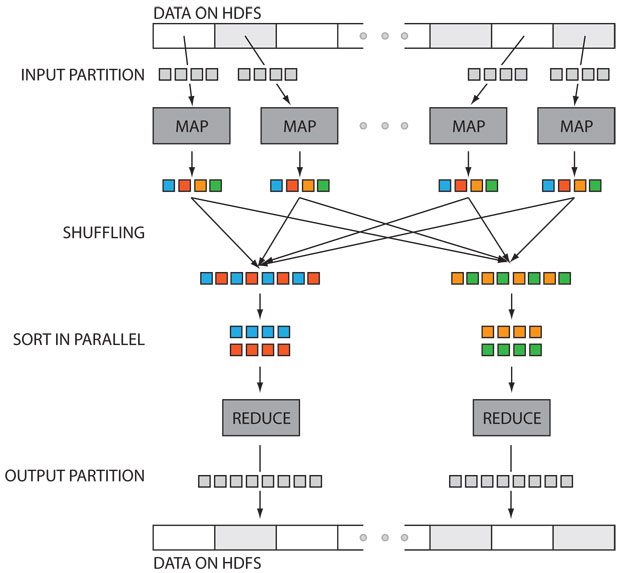
\includegraphics[width=0.4\textwidth]{hadooparch.jpg}
\caption{Hadoop Mapreduce Framework}
\label{fig:hadooparch}
\end{figure}

This model basically has two phase
\begin{enumerate}
\item Map phase
\item Reduce phase
\end{enumerate}

Map phase takes the partitioned input data and converts it into tuples (key value
pairs). There can an optional combiner in the map phase as well. This
is to reduce number of shuffle bytes. This is important because the
primary focus on distributed processing nowadays is to preserve
network bandwidth.

Reduce phase takes output of map phase and reduces to final
output. The framework also takes care of the following
\begin{enumerate}
\item shuffle bytes from map to reducuer
\item Sort all data with the same key
\end{enumerate}

\subsection{Spark}
Spark is an opensource framework for cluster computing developed in
AMPLab at UCBerkeley. It is a generic framework for any large scale
data processing. One of the main idea in spark's design is that most
dataset can fit into RAM. Leveraging this, spark's in memory primitive
makes it 10 to 100 times faster than hadoop mapreduce.

Spark has a primitive in memory data abstraction called Resilient Distributed
Dataset (RDD). RDD has multiple partitions and each partition is
loaded in separate nodes. RDD can be created from any data sources including
HDFS, Cassandra, HBase and S3. RDD Spark provides a set of transformation on
RDD like map, filter, groupBy, sortBy etc. All the transformations
happen parallel on partitions, providing scalability. Since every transformation
is in memory the performance is much faster than Hadoop Mapreduce.

\subsection{Algorithm Design Requirements}

Since these framework are very specific, it is imperative that the
algorithm should be designed to be implemented in one of these
frameworks. Not all algorithms could be readily run on these
frameworks. To design an efficient algorithms for these framworks,
Some of the factors to be considered are

\begin{enumerate}
\item Algorithm has to divide data into partitions and handle the separately
\item There can be common data that can be shared among all the nodes
  but it has to be small
\item Amount of data replication should be minimised. This reduces
  disk IO and increases performance.
\item Amount of data shuffling has to be minimised. This helps in
  preserving network bandwidth
\item Increasing the size of cluster should be able to reduce run time
\end{enumerate}


\section{Algorithm Analysis}
In this section we will review various algorithm and analyse its
suitability for processing huge dataset. we will evaluate various
algorithms based on the following factors.
\begin{enumerate}
\item Size of R and S Datasets ($1 < n < 10^9$)
\item Number of Dimensions ($2 < d < c*10^4$)
\item Horizontal scalability ($1 < nodes < 1000$)
\item Shuffle Bytes
\item Time to complete
\item Accuracy of results
\end{enumerate}

\bigskip
\subsection{iDistance}
One of the early works on KNN Join is \cite{jagadish_idistance:_2005}, in which the authors
introduce a distance based indexing called as iDistance. By using
distance as a measure n dimensional data is converted into single
dimension. They have also used B+ tree as the underlying structure for indexing. By using B+ tree, the
algorithm can be potentially implemented over existing relational databases.

\bigskip
The iDistance algorithm is based on the two key ideas
\begin{enumerate}
\item If two points are similar then they will be similar to a
  reference point as well
\item Can convert any n dimensional point to single dimension by using
  the distance to the reference point
\end{enumerate}

The distance function employed is euclidean. We can use other methods
like hamming, manhattan as well. The euclidean distance between two
points p1 = $(x_0, x_1, ... , x_d)$ and p2 = $(y_0, y_1, ..., y_d)$

\bigskip
dist(p1, p2) = $\sqrt{(x_0 - y_0)^2 + (x_1 - y_1)^2 + ... (x_d - y_d)^2}$
\bigskip

In iDistance algorithm, has following steps for creating the index
\begin{enumerate}
\item N pivots $O_0, O_1 ... O_n$ are chosen either randomly or by finding N clusters'
  center point / edge point.
\item The entire dataset is divided into N partition by finding the
  closest pivot to the point
\item For each point an index key y is obtained by
$y = i*c + dist(p, O_i)$, where c is a constant to make y from
different partition non overlapping
\item Create a B+ Tree to index the transformed points and also create
  an array to store the m pivots with smallest and largest distance
\end{enumerate}

\bigskip

Steps for querying Nearest Neighbours for point q are
\begin{enumerate}
\item Select a $\delta{x}$ as query distance
\item Find partitions that are overlapping with q + $\delta{x}$ as
  radius
\item For the selected partition search for K Nearest neighbours, if
  found stop else increase the $\delta{x}$ and continue step 2 and
  3.
\end{enumerate}

\bigskip
The advantage of this algorithm is that it can be used for both
approximate and accurate calculations by controlling the query
distance $\delta{x}$.

Some of the drawbacks for this algorithm are
\begin{enumerate}
\item This algorithm is designed for point queries (Size of R
  is very small). If two points P1 and P2 are very close in R, we donot reuse the query
distance calculation of P1 for P2
\item For a large dataset calculating the pivots using clustering algorithm are
  computationally intensive themselves
\item Cannot be used in Mapreduce or Spark readily. The main reason being this
  was designed before the age of big data.
\end{enumerate}

\bigskip

\subsection{Analysis: iJoin}
In \cite{yu_efficient_2007}, the authors worked on improving
\cite{jagadish_idistance:_2005}. They solved the drawback 1 stated
above with their algorithm called iJoin. In this method they the
partitioned both R and S dataset and using same pivots and
calculating the probable partition for neighbours in S is found for each
partition of R rather than each point in R. This reduced the
computational complexity to a great extent.

\bigskip

The authors also propose two optimisation and they call it as iJoinAC
and iJoinDR. These two optimisations are primarily to reduce the
number of floating point calculations done if the number of dimensions
are very high, in the order of 1000s. In iJoinAC each datapoint in R
and S are represented by an approximate bounding cube. The iDistance
index is calculated for the bounding cube and when traversal is done
the calculation is simpler and filter out most false answers before we
access the real vectors. The fig ~\ref{fig:iJoinAC} is taken from the original
paper itself.

\begin{figure}[here]
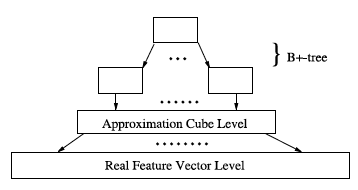
\includegraphics[width=0.4\textwidth]{iJoinAC.png}
\caption{iDistance structure with approximate cube}
\label{fig:iJoinAC}
\end{figure}

In iJoinDR, the dimensions are reduced by applying PCA for the vectors
and choosing the few dimensions. The resulting low dimension vectors
are used for constructing the iDistance index. For example a well
known PCA algorithm called SVD has a computational complexity of
$O(N * d^2)$ where N is the number of datapoints and d number of
dimensions.
\bigskip
As its predecessor, the algorithm is not designed for distributed
datasets. The use of PCA in iJoinDR requires a significant increase in
computation if the dataset is huge. There is no study being done on
impact of approximate PCA results on the algorithm. This would have
helped in reducing the computational complexity for calcuating the
PCA.

Since the algorithm relies heavily on random IO access due to
indexing, adopting the algo to the hadoop mapreduce framework will
difficult because of its sequential design.

There is no easy way to use spark readily for creating indexed
data. Hence this algorithm cannot be readily adapted to spark.

\bigskip

\subsection{Analysis: Gorder}
A great deal of previous research on KNN Join focussed on creating
index for the S dataset, but this paper \cite{xia_gorder:_2004} introduces a
way to optimize the block nested loop join using a method called
GORDER, in which they introduce a new ordering called as grid order.

Grid order partitions the dataspace into $l^d$ rectangular cells where
l is number of segments per dimension of the grid. Two points $p_m <
p_n $ if and only if $v_m < v_n$ where $v_m, v_n$ are cells
surrounding $p_m\ and\ p_n$. $v_m < v_n$ if and only if $v_m(s_k) <
v_n(s_k)$ for dimension k and $\forall\ j < k$
\bigskip

In GORDER algorithm, there are two phases
\begin{enumerate}
\item Compute the PCA for both dataset R and S
\item Sort the dataset based on grid order. The resulting dataset is
  grouped into $l^d$ cells, where l is number of segment per
  dimension.
\item Now for each block in R, probable block in S is selected and KNN
  is calculated within the points in those blocks.
\end{enumerate}

\bigskip

Their approach to solve the high dimensionality problem is
by applying Principal Component Analysis to reduce the dimensions. As
mentioned above the major drawback is that calculating PCA and fory
large datasets is not a feasible solution for a large dataset. There
is no study of effect of approximate PCA on the results.

One another performance reducer of this algorithm in large dataset is that sort
of the whole dataset.

This paper also suffers from the same problem as
\cite{yu_efficient_2007} with regards to its probable adoption to
mapreduce framework.

\bigskip
\subsection{Analysis: zKNN}
In the most recent paper \cite{zhang_efficient_2012}, the authors work on using
MapReduce framework to do parallel KNN Join. In this paper they
describe three algorithms. One very basic algorithm they describe is
called Block Nested Loop Join (BNLJ). In this they partition the R and S
dataset into n partitions and they create $n^2$ buckets
with all combination of R and S partitions. Though this algorithm is
distributed and can run on Hadoop mapreduce framework, this algorithm
performs poorly in all fronts, CPU, Network IO and Disk IO. This is
because the we need have every combination of S and R as possible
which means data replication and transfer of data across nodes. this
is slowest algorithm possible, with complexity of algorithm to be
$O(|R| \times |S|)$

\bigskip

The next algorithm they talk about is Block Nested Loop Join with R
tree index (BRJ). This improves over the Block Nested Loop Join by using R
tree for each S Partition. R tree gives a very good performance for
lower dimensions and it has been used highly effective for lower
dimension \cite{kuan_fast_1997} but for higher dimensions the
performance is almost as bad as a linear scan.

The complexity of the BRJ algorithm is $O(n|S|log(|S|/n) + n|R|\sqrt{|S|/n})$
Though this is better than the BLNJ,
the shuffle bytes and need to bulk load the R tree index and number of
servers needed is high to be used in any practical implementations.

\bigskip

The same paper they also present an approximate algorithm called zKNN
in Hadoop Mapreduce Framework. zKNN is based on mapping
multi-dimensional data into one dimension using space filling
curves. It was initially described for relational databases in \cite{yao_k_2010}
The fig is taken from \cite{song_solutions_2015}

\begin{figure}[here]
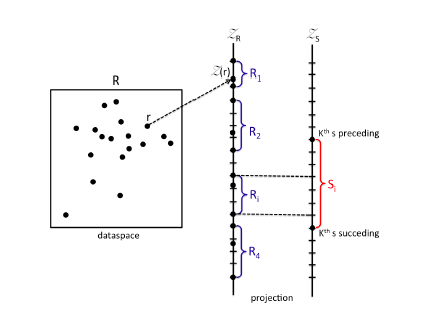
\includegraphics[width=0.4\textwidth]{zknn.png}
\caption{zvalue based partitioning}
\label{fig:zknn.png}
\end{figure}

\bigskip

In zKNN algorithm has the following steps
\begin{enumerate}
\item Transform the data in R and S into single dimension using z order
  curves.
\item Sort and Partition the data in R and S such that the Ri and Si
  has same partition and is sent to same reducers.
\item
\end{enumerate}

\bigskip

The main advantage of the algorithm is its simplicity and is much
faster than other algorithms in map reduce framework
\cite{lu_efficient_2012},
\cite{stupar_rankreduceprocessing_2010}. Also unlike BRJ algorithm it
does not require $n^2$ reducers but only n reducers.

Some of the drawbacks of this algorithm evaluated in
\cite{song_solutions_2015} are
\begin{enumerate}
\item Provides only approximate results
\item Accuracy decreases with increasing dimensions. With 30 dimensions
  accuracy is only 60 percent
\item Accuracy decreases with increased data size
\item The amount of shuffle bytes is approximately 10 times the
  original data and has non linear increase with increasing dimensions, accuracy and
  number of neighbours
\item The study has not covered the impact of very high dimensions
  (100s of dimensions) on the accuracy and how to improve it.
\item It is difficult to add an incremental updates to this algorithm
  as it will require to alter the partitions.
\end{enumerate}

\bigskip

\subsection{Analysis: Rankreduce}

During the same time another study
\cite{stupar_rankreduceprocessing_2010} also focused on getting
approximate KNN Join results in map reduce framework.

This algorithm implements the Distributed Locality Sensitive Hashing (LSH)
based index within Mapreduce framework. LSH uses Locality sensitive
Hash functions which transforms any vectors or objects in d
dimensional space with high probability to a hash bucket.

\bigskip

High level steps for this algorithm is
\begin{enumerate}
\item For every point in S dataset, apply Locality sensitive hash
  functions and add it to a hash bucket
\item For every point in R dataset, apply the same hash functions and
  find the hash bucket
\item Find the nearest Neighbour by computing the distance to every
  element in the bucket
\end{enumerate}


\begin{figure}[here]
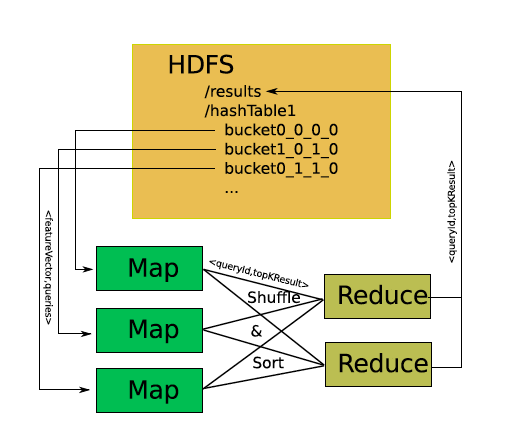
\includegraphics[width=0.4\textwidth]{rankreduce.png}
\caption{RankReduce Framework}
\label{fig:rankreduce.png}
\end{figure}

\bigskip

The advantage of this algorithm is
\begin{enumerate}
\item Simplicity
\item Better accruacy with increasing dataset
\end{enumerate}

\bigskip

The paper in itself does not talk about the following
\begin{enumerate}
\item Effect of high dimension on its accuracy
\item Effect of high dimension on its shuffle bytes
\item Effect of high dimension on its cpu time
\item Effect of number of neighbours on cputime, accuracy
\item Number of hash buckets in relation to dataset size
\item Number of hash buckets to its accuracy
\item Leverage more nodes for parallel processing
\end{enumerate}

Though the algorithm looks promising in the space of approximate KNN
Join algorithm, still more work needs to be done in order to properly
compare with \cite{zhang_efficient_2012}. On the other hand the
evaluation by \cite{song_solutions_2015} shows that though
\cite{zhang_efficient_2012} has better performance than
\cite{stupar_rankreduceprocessing_2010}, it has lower accuracy.
\bigskip
\subsection{Analysis: Voronoi Partition}
Though mapreduce framework has been around for nearly 10 years, there
is only one KNN Join algorithm \cite{lu_efficient_2012} which is
optimized for the mapreduce framework and that provides accurate
results.

This algorithm is based on voronoi partition. The algorithm is
divided into 4 Phases
\begin{enumerate}
\item Preprocessing phase: In this phase pivots are selected
\item Data Partitioning Phase: In this phase both R and S dataset is
  partitioned based on the nearest pivot.
\item Join Map Phase: In this phase data points in S is replicated to
  all partitions of R
\item Join Reduce Phase: Nearest neighbours are found based on data
  for each partition
\end{enumerate}

\bigskip

In the preprocessing phase we select the pivots. The paper
investigates on three different ways to select the pivots.
\begin{enumerate}
\item Random Selection
\item Farthest Selection
\item K Means Selection
\end{enumerate}

Farthest Selection is worthless in every aspect of performance and
selectivity. Though K Means selection results in better selectivity of partition
and therefore faster computation in Phase 3 and 4, preprocessing time
is slower. Random selection is relatively results in faster
preprocessing time than K Means, but both of them take a significant
amount of time. The computation cost of Random Selection is $O(n^2)$
where n is the number of pivots. This preprocessing phase does not use the
mapreduce framework at all. It would be more efficient if we use map
reduce for this phase as well. One possible way is given in
\cite{kiefer_pairwise_2010}.

\bigskip

Data partitioning phase has two objectives.
\begin{enumerate}
\item Divide the data into parititions in both R and S dataset
\item Generate Summary Table which contains number of elements in each
  partitions, minimum and maximum distance of points from the pivot, K
  Nearest Neighbours of pivots and their distance
\end{enumerate}

The computation cost of this phase is $O(|S|*n + |R|*n)$ where n is
the number of pivots. Higher the number of pivots results in longer
data partitioning phase but results in smaller partition. Smaller
parition will be easier to compute the KNN for a partition.

There is a scope for improving ther performance of this phase by
leveraging either iDistance indexing \cite{jagadish_idistance:_2005}
or creating a custom range trees or kd trees.

\bigskip

In Join Map Phase, there are 2 different steps
\begin{enumerate}
\item For each partition in R, bounding Region in S is computed. The
  computational complexity is $O(n^2)$ where n is the number of
  partitions. The Summary table generated in previous data
  partitioning phase is used as input.
\item For every point in S, if it is in bounding Region for a
  partition $R_i$, data is replicated to that partition $R_i$. In this way
  every partition $R_i$ in Join Reduce Phase gets all the probable
  points in S that could be a neighbour for a point in $R_i$
\end{enumerate}

The computation complexity of step 2 is $O(|S| * n)$ where n is the
number of partitions. If the number of paritions is less then
partition pruning will be poor. This phase also generates more shuffle
bytes. It also depends on number of dimensions. If the number of
dimensions is 10 and number of partition is 2000, the data replication
is around 80 times. This is one of the primary reason for poor
performance of this algorithm.

\bigskip

In Join Reduce phase, each reducer gets all points from $R_i$ and all
probable points from S. Now we compute the plain KNN for partition
$R_i$.

This algorithm performs better than BNLJ or BRJ.

% An example of a floating figure using the graphicx package.
% Note that \label must occur AFTER (or within) \caption.
% For figures, \caption should occur after the \includegraphics.
% Note that IEEEtran v1.7 and later has special internal code that
% is designed to preserve the operation of \label within \caption
% even when the captionsoff option is in effect. However, because
% of issues like this, it may be the safest practice to put all your
% \label just after \caption rather than within \caption{}.
%
% Reminder: the "draftcls" or "draftclsnofoot", not "draft", class
% option should be used if it is desired that the figures are to be
% displayed while in draft mode.
%
%\begin{figure}[!t]
%\centering
%\includegraphics[width=2.5in]{myfigure}
% where an .eps filename suffix will be assumed under latex,
% and a .pdf suffix will be assumed for pdflatex; or what has been declared
% via \DeclareGraphicsExtensions.
%\caption{Simulation results for the network.}
%\label{fig_sim}
%\end{figure}

% Note that IEEE typically puts floats only at the top, even when this
% results in a large percentage of a column being occupied by floats.


% An example of a double column floating figure using two subfigures.
% (The subfig.sty package must be loaded for this to work.)
% The subfigure \label commands are set within each subfloat command,
% and the \label for the overall figure must come after \caption.
% \hfil is used as a separator to get equal spacing.
% Watch out that the combined width of all the subfigures on a
% line do not exceed the text width or a line break will occur.
%
%\begin{figure*}[!t]
%\centering
%\subfloat[Case I]{\includegraphics[width=2.5in]{box}%
%\label{fig_first_case}}
%\hfil
%\subfloat[Case II]{\includegraphics[width=2.5in]{box}%
%\label{fig_second_case}}
%\caption{Simulation results for the network.}
%\label{fig_sim}
%\end{figure*}
%
% Note that often IEEE papers with subfigures do not employ subfigure
% captions (using the optional argument to \subfloat[]), but instead will
% reference/describe all of them (a), (b), etc., within the main caption.
% Be aware that for subfig.sty to generate the (a), (b), etc., subfigure
% labels, the optional argument to \subfloat must be present. If a
% subcaption is not desired, just leave its contents blank,
% e.g., \subfloat[].


% An example of a floating table. Note that, for IEEE style tables, the
% \caption command should come BEFORE the table and, given that table
% captions serve much like titles, are usually capitalized except for words
% such as a, an, and, as, at, but, by, for, in, nor, of, on, or, the, to
% and up, which are usually not capitalized unless they are the first or
% last word of the caption. Table text will default to \footnotesize as
% IEEE normally uses this smaller font for tables.
% The \label must come after \caption as always.
%
%\begin{table}[!t]
%% increase table row spacing, adjust to taste
%\renewcommand{\arraystretch}{1.3}
% if using array.sty, it might be a good idea to tweak the value of
% \extrarowheight as needed to properly center the text within the cells
%\caption{An Example of a Table}
%\label{table_example}
%\centering
%% Some packages, such as MDW tools, offer better commands for making tables
%% than the plain LaTeX2e tabular which is used here.
%\begin{tabular}{|c||c|}
%\hline
%One & Two\\
%\hline
%Three & Four\\
%\hline
%\end{tabular}
%\end{table}


% Note that the IEEE does not put floats in the very first column
% - or typically anywhere on the first page for that matter. Also,
% in-text middle ("here") positioning is typically not used, but it
% is allowed and encouraged for Computer Society conferences (but
% not Computer Society journals). Most IEEE journals/conferences use
% top floats exclusively.
% Note that, LaTeX2e, unlike IEEE journals/conferences, places
% footnotes above bottom floats. This can be corrected via the
% \fnbelowfloat command of the stfloats package.

\bigskip

\section{Conclusion}

Though there are few algorithms which are implemented in mapreduce
framework, they are far from efficient for a large dataset. And
moreover they are not designed for efficient network bandwidth
utilisation. None of the algorithm is designed for spark framework.

% trigger a \newpage just before the given reference
% number - used to balance the columns on the last page
% adjust value as needed - may need to be readjusted if
% the document is modified later
%\IEEEtriggeratref{8}
% The "triggered" command can be changed if desired:
%\IEEEtriggercmd{\enlargethispage{-5in}}

% references section
\newpage
% can use a bibliography generated by BibTeX as a .bbl file
% BibTeX documentation can be easily obtained at:
% http://www.ctan.org/tex-archive/biblio/bibtex/contrib/doc/
% The IEEEtran BibTeX style support page is at:
% http://www.michaelshell.org/tex/ieeetran/bibtex/
\bibliography{knnjoin}
\bibliographystyle{IEEEtran}
% argument is your BibTeX string definitions and bibliography database(s)

%
% <OR> manually copy in the resultant .bbl file
% set second argument of \begin to the number of references
% (used to reserve space for the reference number labels box)
% \begin{thebibliography}{1}

% \bibitem{IEEEhowto:kopka}
% H.~Kopka and P.~W. Daly, \emph{A Guide to \LaTeX}, 3rd~ed.\hskip 1em plus
%   0.5em minus 0.4em\relax Harlow, England: Addison-Wesley, 1999.

% \end{thebibliography}




% that's all folks
\end{document}

%%% Local Variables:
%%% mode: latex
%%% TeX-master: t
%%% End:
